\documentclass{./../../Latex/tests}

\begin{document}
\thispagestyle{plain}
\myheader{Sample 1: Midterm Exam}
\rhead{Sample 1: Midterm Exam}
\vspace{0.5em}
\testHeader{70}{20}


\underline{Question 1: Multiple Choice Questions (1 pt each, total 5 pts)}

Select one correct answer unless specified otherwise.
\begin{enumerate}
\item[(a).]	 Below is a scatter plot of two variables $X$ and $Y$. \\
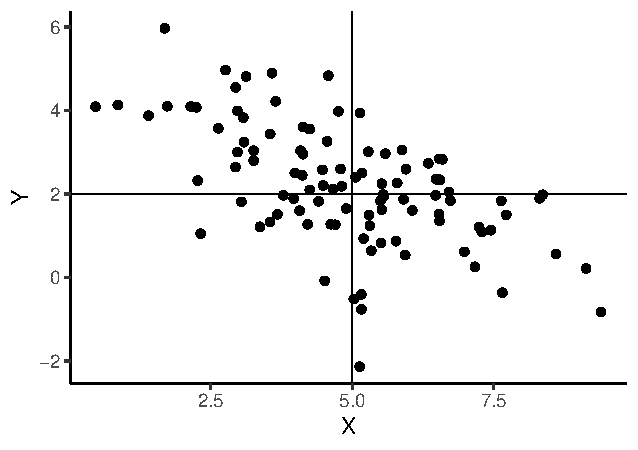
\includegraphics{./../../output/corr_midterm.pdf}\\
What is the correlation between these variables?
\begin{enumerate}
\item[$\square$] $\rho = 0.4$
\item[$\square$] $\rho = -1$
\item[$\square$] $\rho = -0.6$
\item[$\square$] $\rho = 0$ \\
\end{enumerate}
%\item[(b).] (Select all that apply) Suppose a survey of 500 people found that 300 of them prefer coffee over tea. Suppose we define a variable X that takes a value of 1 if a person said they prefer coffee and 0 otherwise. The sample mean of $X$ is given as:
%\begin{enumerate}
%\item[$\square$] $1/500(1\cdot 300 + 0\cdot 200) $ 
%\item[$\square$] $(1/500)\sum_{i=1}^{500} X_i$
%\item[$\square$] $300/500$
%\item[$\square$] $1\cdot (3/5) + 0\cdot (2/5) $ \\
%\end{enumerate}
\item[(b).] If the average height in the world is 169 cm with a standard deviation of 6 cm, and my height is 167 cm, how many standard deviations below the mean am I?
\begin{enumerate}
\item[$\square$] $1.24$
\item[$\square$] $0.33$
\item[$\square$] $0.67$
\item[$\square$] $2.82$ \\
\end{enumerate}
\newpage
\item[(c).] $X$ and $Y$ are two \textit{independent} random variables. $X$ is a binary variable that takes the value 1 or 0, and $Y$ is a continuous variable. We know that $E(Y|X=1) = 100$, then:
\begin{enumerate}
\item[$\square$] $E(Y|X=0) = 50$
\item[$\square$] $E(Y|X=0) = 100$
\item[$\square$] $E(Y|X=0) = 200$
\item[$\square$] We can't say anything about $E(Y|X=0)$ with the above information. \\
\end{enumerate}
\item[(d).] Sample mean $\bar{X}$ is an unbiased estimator for the true population mean $\mu$. Does this mean
\begin{enumerate}
	\item[$\square$] $\bar{X}=\mu$ in all samples.
	\item[$\square$] $\bar{X}=\mu$ on average across samples.
	\item[$\square$] $E(\bar{X})=0$
	\item[$\square$] All of the above \\
\end{enumerate}
\item[(e).] (Select all that apply.) Which of the following statements about confidence intervals is true?
\begin{enumerate}
	\item[$\square$] The confidence interval widens as the population variance decreases.
	\item[$\square$] The confidence interval widens as the population variance increases.
	\item[$\square$] The confidence interval widens as the sample size decreases.
	\item[$\square$] The confidence interval widens as the sample size increases. \\
\end{enumerate}
\end{enumerate}


\newpage
\underline{Question 2: Things you can explain (6 pts)} \\
\begin{enumerate}
\item[(a).] (2 pts) In most countries across the world, mean earnings are greater than median earnings. Why do you think this is true?  
\vspace{4.5cm}
\item[(b).] (2 pts) There is a strong positive correlation between immigrant flows and online job vacancies across metropolitan areas in the US. Does this imply that immigration leads to job creation? 
\vspace{4.5cm}
\item[(c).] (2 pts) As long as our sample is random (no matter how small or large), the sample mean is going to give us an unbiased estimate of the true population mean. Why do we still care about having a large sample?
\end{enumerate}

\newpage 
\underline{Question 3: Voter Turnout (9 pts)} \\

 We took a random sample of 200 individuals from the US population and asked them whether they voted in the last 
election. We then create a variable $X_i$ that takes value 1 if the individual
voted in the last election and 0 if they did not. 140 individuals said they voted in the last election, while 60 individuals said they didn't. This data is presented in the table below.\\  
\begin{center}
\setstretch{2}
\begin{tabularx}{\textwidth}{@{}Y| @{}Y |@{}Y| @{}Y| @{}Y| @{}Y@{}}
$(1)$ & $(2)$ & $(3)$ & $(4)$ & $(5)$ & $(6)$ \\
 $X_i$ & $n_i$ & $f_i$ & $f_i X_i$ & $(X_i-\bar{X})^2$ & $f_i (X_i-\bar{X})^2$ \\  \hline
 1 & 140 & & & & \\ \hline
 0 & 60 & & & & \\ \hline
Total & 200 & & & NA & \\ 
\end{tabularx}	
\end{center}
\vspace{2em}


 \begin{enumerate}
 \item[(a).] (2 pts) Fill in the third and the fourth column of the above frequency distribution table and calculate $\bar{X}$,  the sample mean of $X_i$. Specify the formula you will use and then plug in the values to calculate your answer. 
\newpage
\item[(b).] (2 pts) Your answer in (a) tells us the proportion of individuals in our sample who voted in the last election. Can we directly infer the percentage of the US population that voted in the last election from this answer? Explain. \\~\\
\vspace{6cm} \\
\item[(c).] (2 pts) Fill in the fifth and the sixth column of the above frequency distribution table and calculate $S^2_X$,  the sample variance of $X_i$. Specify the formula you will use and then plug in the values to calculate your answer. 
\newpage
\item[(d).] (2 pts) Construct a 90\% confidence interval for voter turnout in the U.S. population.

Note: $Pr(Z>1.645) = 0.05$, $Pr(Z>1.96) = 0.025$, $Pr(Z>2.33) = 0.01$
 
\vspace{6cm}

\item[(e).] (1 pt) Interpret the confidence interval you’ve constructed in part (d). What does it reflect in this case? 
\end{enumerate}






\end{document}